\documentclass{report}
% Include all project wide packages here.
\usepackage{fullpage}
\usepackage[style=ieee]{biblatex}
\usepackage[dutch]{babel}

\renewcommand{\familydefault}{\sfdefault}

\setmainfont[Ligatures=TeX]{Myriad Pro}
\setmathfont{Asana Math}
\setmonofont{Lucida Console}

\usepackage{titlesec, blindtext, color}
\definecolor{gray75}{gray}{0.75}
\newcommand{\hsp}{\hspace{20pt}}
\titleformat{\chapter}[hang]{\Huge\bfseries}{\thechapter\hsp\textcolor{gray75}{|}\hsp}{0pt}{\Huge\bfseries}
\renewcommand{\familydefault}{\sfdefault}
\renewcommand{\arraystretch}{1.2}
\setlength\parindent{0pt}

%For code listings
\definecolor{black}{rgb}{0,0,0}
\definecolor{browntags}{rgb}{0.65,0.1,0.1}
\definecolor{bluestrings}{rgb}{0,0,1}
\definecolor{graycomments}{rgb}{0.4,0.4,0.4}
\definecolor{redkeywords}{rgb}{1,0,0}
\definecolor{bluekeywords}{rgb}{0.13,0.13,0.8}
\definecolor{greencomments}{rgb}{0,0.5,0}
\definecolor{redstrings}{rgb}{0.9,0,0}
\definecolor{purpleidentifiers}{rgb}{0.01,0,0.01}


\lstdefinestyle{csharp}{
language=[Sharp]C,
showspaces=false,
showtabs=false,
breaklines=true,
showstringspaces=false,
breakatwhitespace=true,
escapeinside={(*@}{@*)},
columns=fullflexible,
commentstyle=\color{greencomments},
keywordstyle=\color{bluekeywords}\bfseries,
stringstyle=\color{redstrings},
identifierstyle=\color{purpleidentifiers},
basicstyle=\ttfamily\small}

\lstdefinestyle{c}{
language=C,
showspaces=false,
showtabs=false,
breaklines=true,
showstringspaces=false,
breakatwhitespace=true,
escapeinside={(*@}{@*)},
columns=fullflexible,
commentstyle=\color{greencomments},
keywordstyle=\color{bluekeywords}\bfseries,
stringstyle=\color{bluestrings},
identifierstyle=\color{purpleidentifiers}
}

\lstdefinestyle{vhdl}{
language=VHDL,
showspaces=false,
showtabs=false,
breaklines=true,
showstringspaces=false,
breakatwhitespace=true,
escapeinside={(*@}{@*)},
columns=fullflexible,
commentstyle=\color{greencomments},
keywordstyle=\color{bluekeywords}\bfseries,
stringstyle=\color{redstrings},
identifierstyle=\color{purpleidentifiers}
}

\lstdefinestyle{xaml}{
language=XML,
showspaces=false,
showtabs=false,
breaklines=true,
showstringspaces=false,
breakatwhitespace=true,
escapeinside={(*@}{@*)},
columns=fullflexible,
commentstyle=\color{greencomments},
keywordstyle=\color{redkeywords},
stringstyle=\color{bluestrings},
tagstyle=\color{browntags},
morestring=[b]",
  morecomment=[s]{<?}{?>},
  morekeywords={xmlns,version,typex:AsyncRecords,x:Arguments,x:Boolean,x:Byte,x:Char,x:Class,x:ClassAttributes,x:ClassModifier,x:Code,x:ConnectionId,x:Decimal,x:Double,x:FactoryMethod,x:FieldModifier,x:Int16,x:Int32,x:Int64,x:Key,x:Members,x:Name,x:Object,x:Property,x:Shared,x:Single,x:String,x:Subclass,x:SynchronousMode,x:TimeSpan,x:TypeArguments,x:Uid,x:Uri,x:XData,Grid.Column,Grid.ColumnSpan,Click,ClipToBounds,Content,DropDownOpened,FontSize,Foreground,Header,Height,HorizontalAlignment,HorizontalContentAlignment,IsCancel,IsDefault,IsEnabled,IsSelected,Margin,MinHeight,MinWidth,Padding,SnapsToDevicePixels,Target,TextWrapping,Title,VerticalAlignment,VerticalContentAlignment,Width,WindowStartupLocation,Binding,Mode,OneWay,xmlns:x}
}

%defaults
\lstset{
basicstyle=\ttfamily\small,
extendedchars=false,
numbers=left,
numberstyle=\ttfamily\tiny,
stepnumber=1,
tabsize=4,
numbersep=5pt
}
\addbibresource{../../library/bibliography.bib}

\title{EPO-2: Mid-term Design Report - Mijndetector}
\author{Chy Lau}

\begin{document}

\chapter{Mijndetector}
\label{ch:mijn}
%DONE: take out why inductive over capacitive
Om een mijndetector op te bouwen, moet er eerst een keuze worden gemaakt tussen de verschillende soorten sensoren. Maken we gebruik van een inductieve sensor, capacitieve sensor of een combinatie van beide? 

Een inductieve sensor werkt op basis van de verandering van magnetische permeabiliteit. De inductantie van de spoel verandert, wat leidt tot een verandering van de resonantiefrequentie van het bijbehorende circuit.

Een capacitieve sensor werkt op basis van de verandering van capaciteit. Door de aanwezigheid van de mijn verandert de capaciteit van een condensator, wat leidt tot een verandering van de spanning. 

\section{Eisen}
\label{sec:eisen}
De mijn-detecterende sensor moet aan de volgende eisen voldoen: 
%DONE: More specific i.e. between 5 V and 0 V.
%DONE: Detection range: ~2.15 cm
\begin{itemize}
\item De mijndetector moet een metalen ring van 3 cm \diameter op een afstand van \~2 cm detecteren op het wedstrijdveld
\item De sensor mag geen contact maken met de metalen ring
\item De sensor moet op een voedingsspanning van 5 V en 0 V werken
\item Het uitgangssignaal van de sensor is een blokgolf met een maximum waarde van 5 V en een minimum waarde van 0 V
\end{itemize}

\section{Ontwerp}
\label{sec:ontwerp}
%DONE: dezelfde configuratie als JIT, maar andere waarden
%DONE: Add why inductive sensor
We hadden eerst voor een capacitieve sensor gekozen. Echter toen werkte de schakeling van de sensor niet; de oscilloscoop gaf geen signaal weer. Dus hebben we voor de inductieve sensor gekozen.

De schakeling van de inductieve sensor is op basis van de JIT: Inductieve sensoren gemaakt. De configuratie is hetzelfde, maar er zijn andere waarden voor de componenten gebruikt. In figuur \ref{fig:schakeling_sensor} staat de oscillator op basis van de inductieve sensor.

\subsection{Werkingsprincipe}
\label{ssec:werking}
Over het algemeen zijn er twee mogelijke werkingsprincipes voor de inductieve sensor. De eerste werkt op basis van de verandering van permeabiliteit. De tweede werkt op basis van een pulserend veld. 

Voor de sensor geldt het eerste werkingsprincipe. Er zal een verschil van magnetische permeabiliteit gedetecteerd worden, omdat lucht een andere permeabiliteit heeft dan metaal. De magnetische veldlijnen uit de spoel zullen veranderd worden wanneer ze door het metaal heen gaan. Dit leidt ertoe dat de inductiviteit van de spoel verandert. Deze verandering kan worden weergegeven in een periodiek signaal.

\newpage
\subsection{Werking}

%DONE:resonatie circuit ->permeabiliteit verandert van spoel->frequentie verandert
De schakeling die gebruikt wordt voor de inductieve sensor is een resonant LC-circuit. Wanneer de permeabiliteit verandert, zal ook de inductantie van de spoel veranderen. Hierdoor wijzigt de resonantiefrequentie en dus ook het uitgangssignaal.

\begin{figure}[H]
\centering
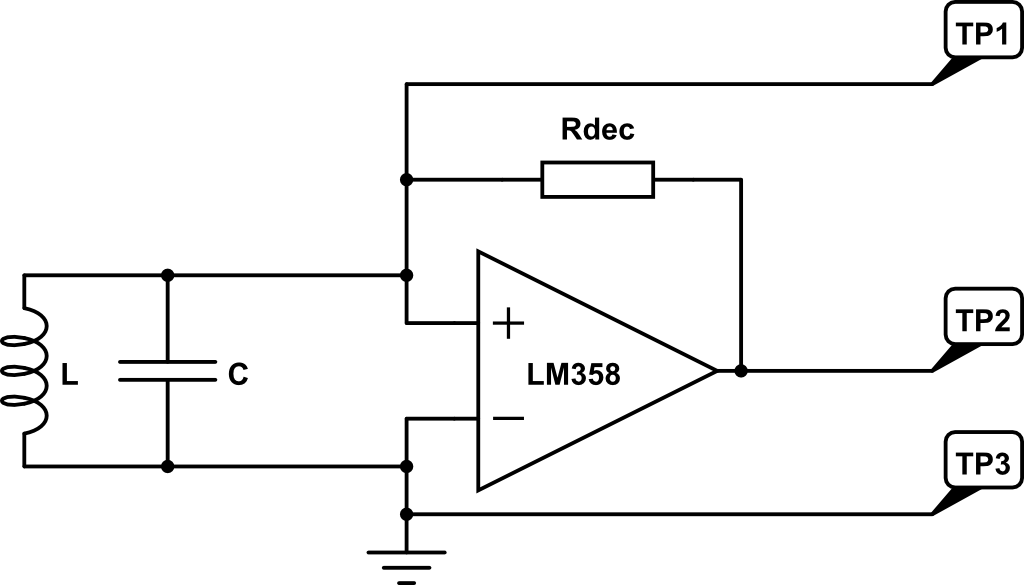
\includegraphics[scale=0.45]{inductieve_sensor.png}
\caption{Schakeling van de inductieve sensor.}
\label{fig:schakeling_sensor}
\end{figure}

\subsubsection{LC-circuit}
%Good!
Een belangrijke eigenschap van het circuit is de resonantiefrequentie. Om $f_{res}$ te begrijpen is het van belang om naar het gedrag van de elektronen te kijken. De elektronen schommelen steeds heen en weer, van de ene kant van de condensator-plaat naar de andere kant van de condensator-plaat. Hoe snel zo een schommeling gaat, wordt uitgedrukt als de resonantiefrequentie. Deze frequentie hangt af van de spoel en condensator die worden gebruikt in het circuit. Met de volgende formule kan$f_{res}$ worden berekend:

\begin{equation}
f_{res}=\frac{1}{2\pi\sqrt{LC}}
\end{equation}

\subsubsection{Comparator}
%Good!
De comparator is een essentieel onderdeel van de schakeling. Het zorgt ervoor dat er op een uitgang een blokgolf komt te staan. Zo een blokgolf kan dan getransformeerd worden in een logisch signaal van '0' en '1'. De comparator werkt als volgt:

\begin{equation}
Als \;V_+ > V_- \rightarrow V_{out}\approx V_{CC}
\end{equation}
\begin{equation}
Als \; V_+ < V_- \rightarrow V_{out}\approx V_{EE}
\end{equation}

\noindent
Dit leidt ertoe dat de uitgangsspanning clampt aan twee waarden, de voedingsspanningen van de op-amp, resulterend in een blokgolf. In het circuit voor de mijnendetector variëert de blokgolf dus tussen de 5 V en 0 V.\\

\section{Implementatie}
%Gemeten waarden
Om het ontwerp van de inductieve sensor schakeling te realiseren, werd de schakeling eerst op een breadboard gemaakt. Stel dat er problemen zijn met het ontwerp, dan is het mogelijk om de schakeling te wijzigen. Als er meteen gesoldeerd wordt, is er een grote kans dat de schakeling het niet meteen doet, wat resulteert in desolderen of het weggooien van werkende componenten.\\ 

\noindent Voor het circuit zijn de volgende componenten gebruikt:
\begin{itemize}
\item 1$\times$ spoel: $4.7 \mathrm{mH}$
\item 1$\times$ condensator: $30 \mu \mathrm{F}$
\item 1$\times$ op-amp: LM358
\item 1$\times$ weerstand: $820 \Omega$
\end{itemize}

\noindent
De waarden zijn bepaald door middel van trial and error. Voor de weerstand in de feedback-configuratie is ervan uitgegaan dat de waarde niet te groot mag zijn, want dan loopt er geen stroom meer terug om de oscillatie in stand te houden. Een waarde van 10 k$\Omega$ zou te groot zijn; het moest rond de 1 k$\Omega$ zijn.

De afmeting van de spoel was het belangrijkste om rekening mee te houden. Er is gekozen voor een spoel met ongeveer dezelfde diameter, zodat de sensor ongeveer een detectie afstand van 2 cm heeft. De gemeten afstand is 2.15 cm \pm 0.05 cm (van middelpunt spoel naar middelpunt munt).

De sensor output, een blokgolf van 5 V - 0 V, wordt met VHDL-code omgezet in een bit-signaal. Hierbij is het '0' wanneer er een lage spanning op de uitgang staat en '1' wanneer er een hoge spanning op de uitgang staat. De code voor de VHDL-implementatie staat in de bijlage.

\section{Test}
De inductieve sensor schakeling is als eerste getest. Deze is daarvoor op de oscilloscoop aangesloten met twee probes (1:10) aan de klemmen TP1 en TP2. Bovendien is de aardklem van de oscilloscoop aangesloten op klem TP3. De voeding van de op-amp is op een spanning van +5 V en GND aangesloten. Er kan geen negatieve spanning over de inverterende-ingang van de op-amp worden aangesloten, omdat de batterij op de robot dit niet kan leveren. 

Op de display van de oscilloscoop moet er een blokgolf worden weergegeven. Als het uitgangssignaal geen blokgolf is, kan er meteen vanuit worden gegaan dat er iets mis is met de schakeling, voeding of de instellingen van de oscilloscoop.\\
De berekende waarde van de resonantie frequentie:
$f_{res}=\frac{1}{2\pi \sqrt{4.7\times 10^{-3}\cdot 30\times 10^{-6}}}= 424 \mathrm{Hz}$

\noindent De gemeten waarde van de resonantie frequentie:
$f_{res}\approx400 \mathrm{Hz}$\\

\noindent Het tweede deel van de test-sessie is de implementatie met VHDL. De VHDL-code voor de mijndetector wordt eerst gesimuleerd met behulp van een testbench en daarna gesynthetiseerd zodat het op de FPGA geprogrammeerd kan worden. 

\section{Discussie}
Er is tijdens de projectmiddag veel tijd besteed aan het bouwen van de schakeling. Op de oscilloscoop was het uitgangssignaal van de sensor geen blokgolf. Na enkele keren zorgvuldig de schakeling te hebben gebouwd, is het gelukt om een blokgolf te krijgen. Het probleem werd veroorzaakt doordat de draden niet goed in contact waren met het breadboard.

Verder was het trial and error om de juiste waarde van de gevoeligheid te bepalen. Dit werd gedaan door een metalen munt onder de sensor te schuiven en daarna de gevoeligheid te tweaken, totdat de threshold in de VHDL-code hoog genoeg lag om alleen bij een munt tot een detectie te leiden.

\end{document}